


\tikzset{every picture/.style={line width=0.75pt}} %set default line width to 0.75pt        

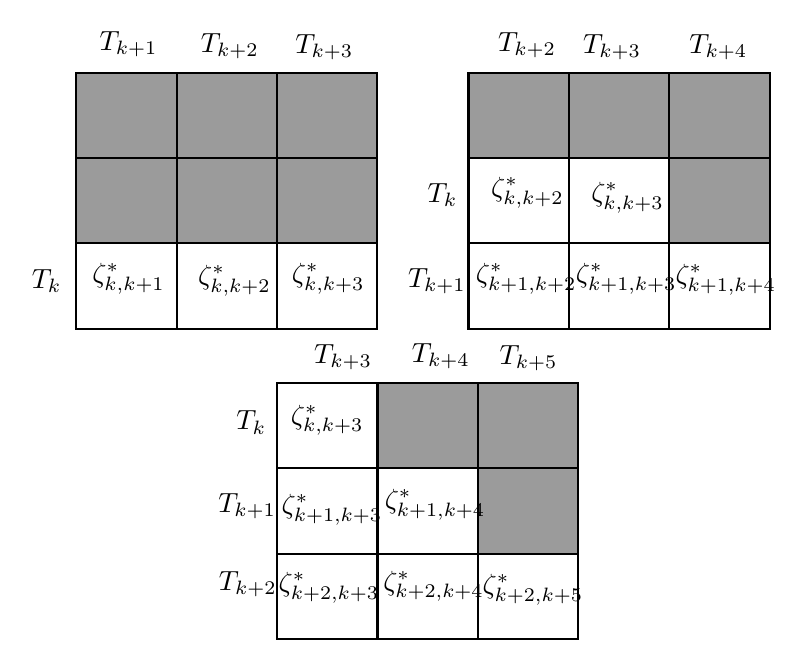
\begin{tikzpicture}[x=0.75pt,y=0.75pt,yscale=-0.8,xscale=0.8]
%uncomment if require: \path (0,596); %set diagram left start at 0, and has height of 596

%Shape: Rectangle [id:dp001467504860766411] 
\draw  [fill={rgb, 255:red, 155; green, 155; blue, 155 }  ,fill opacity=1 ] (75.88,39.44) -- (136.34,39.44) -- (136.34,90.89) -- (75.88,90.89) -- cycle ;
%Shape: Rectangle [id:dp12013579244898587] 
\draw  [fill={rgb, 255:red, 155; green, 155; blue, 155 }  ,fill opacity=1 ] (136.34,39.44) -- (196.79,39.44) -- (196.79,90.89) -- (136.34,90.89) -- cycle ;
%Shape: Rectangle [id:dp15646042985612296] 
\draw  [fill={rgb, 255:red, 155; green, 155; blue, 155 }  ,fill opacity=1 ] (196.79,39.44) -- (257.25,39.44) -- (257.25,90.89) -- (196.79,90.89) -- cycle ;
%Shape: Rectangle [id:dp14798072255631367] 
\draw  [fill={rgb, 255:red, 155; green, 155; blue, 155 }  ,fill opacity=1 ] (136.34,90.89) -- (196.79,90.89) -- (196.79,142.34) -- (136.34,142.34) -- cycle ;
%Shape: Rectangle [id:dp27799179334673507] 
\draw  [fill={rgb, 255:red, 155; green, 155; blue, 155 }  ,fill opacity=1 ] (75.88,90.89) -- (136.34,90.89) -- (136.34,142.34) -- (75.88,142.34) -- cycle ;
%Shape: Rectangle [id:dp27211719867907513] 
\draw  [fill={rgb, 255:red, 155; green, 155; blue, 155 }  ,fill opacity=1 ] (196.79,90.89) -- (257.25,90.89) -- (257.25,142.34) -- (196.79,142.34) -- cycle ;
%Shape: Rectangle [id:dp6135251307737215] 
\draw   (75.88,142.34) -- (136.34,142.34) -- (136.34,193.8) -- (75.88,193.8) -- cycle ;
%Shape: Rectangle [id:dp20310123993966211] 
\draw   (136.34,142.34) -- (196.79,142.34) -- (196.79,193.8) -- (136.34,193.8) -- cycle ;
%Shape: Rectangle [id:dp7690123814029686] 
\draw   (196.79,142.34) -- (257.25,142.34) -- (257.25,193.8) -- (196.79,193.8) -- cycle ;
%Shape: Rectangle [id:dp8019843366921173] 
\draw  [fill={rgb, 255:red, 155; green, 155; blue, 155 }  ,fill opacity=1 ] (312.17,39.44) -- (372.63,39.44) -- (372.63,90.89) -- (312.17,90.89) -- cycle ;
%Shape: Rectangle [id:dp7475312469210154] 
\draw  [fill={rgb, 255:red, 155; green, 155; blue, 155 }  ,fill opacity=1 ] (372.63,39.44) -- (433.09,39.44) -- (433.09,90.89) -- (372.63,90.89) -- cycle ;
%Shape: Rectangle [id:dp6482558063667325] 
\draw  [fill={rgb, 255:red, 155; green, 155; blue, 155 }  ,fill opacity=1 ] (433.09,39.44) -- (493.55,39.44) -- (493.55,90.89) -- (433.09,90.89) -- cycle ;
%Shape: Rectangle [id:dp3420877816265564] 
\draw   (372.63,90.89) -- (433.09,90.89) -- (433.09,142.34) -- (372.63,142.34) -- cycle ;
%Shape: Rectangle [id:dp836363094154154] 
\draw   (312.17,90.89) -- (372.63,90.89) -- (372.63,142.34) -- (312.17,142.34) -- cycle ;
%Shape: Rectangle [id:dp1801360471105331] 
\draw  [fill={rgb, 255:red, 155; green, 155; blue, 155 }  ,fill opacity=1 ] (433.09,90.89) -- (493.55,90.89) -- (493.55,142.34) -- (433.09,142.34) -- cycle ;
%Shape: Rectangle [id:dp3309839576206759] 
\draw   (312.17,142.34) -- (372.63,142.34) -- (372.63,193.8) -- (312.17,193.8) -- cycle ;
%Shape: Rectangle [id:dp6154069784921214] 
\draw   (372.63,142.34) -- (433.09,142.34) -- (433.09,193.8) -- (372.63,193.8) -- cycle ;
%Shape: Rectangle [id:dp2922477144180189] 
\draw   (433.09,142.34) -- (493.55,142.34) -- (493.55,193.8) -- (433.09,193.8) -- cycle ;
%Shape: Rectangle [id:dp6297592399056027] 
\draw   (196.92,226.28) -- (257.38,226.28) -- (257.38,277.73) -- (196.92,277.73) -- cycle ;
%Shape: Rectangle [id:dp9856266195519265] 
\draw  [fill={rgb, 255:red, 155; green, 155; blue, 155 }  ,fill opacity=1 ] (257.38,226.28) -- (317.84,226.28) -- (317.84,277.73) -- (257.38,277.73) -- cycle ;
%Shape: Rectangle [id:dp5718619595286711] 
\draw  [fill={rgb, 255:red, 155; green, 155; blue, 155 }  ,fill opacity=1 ] (317.84,226.28) -- (378.29,226.28) -- (378.29,277.73) -- (317.84,277.73) -- cycle ;
%Shape: Rectangle [id:dp15981629810632536] 
\draw   (257.38,277.73) -- (317.84,277.73) -- (317.84,329.19) -- (257.38,329.19) -- cycle ;
%Shape: Rectangle [id:dp07001551025478414] 
\draw   (196.92,277.73) -- (257.38,277.73) -- (257.38,329.19) -- (196.92,329.19) -- cycle ;
%Shape: Rectangle [id:dp4801148492513494] 
\draw  [fill={rgb, 255:red, 155; green, 155; blue, 155 }  ,fill opacity=1 ] (317.84,277.73) -- (378.29,277.73) -- (378.29,329.19) -- (317.84,329.19) -- cycle ;
%Shape: Rectangle [id:dp4962651822994415] 
\draw   (196.92,329.19) -- (257.38,329.19) -- (257.38,380.64) -- (196.92,380.64) -- cycle ;
%Shape: Rectangle [id:dp029501558482666113] 
\draw   (257.38,329.19) -- (317.84,329.19) -- (317.84,380.64) -- (257.38,380.64) -- cycle ;
%Shape: Rectangle [id:dp23894170190967312] 
\draw   (317.84,329.19) -- (378.29,329.19) -- (378.29,380.64) -- (317.84,380.64) -- cycle ;

% Text Node
\draw (83.77,152.38) node [anchor=north west][inner sep=0.75pt]    {$\zeta ^{*}_{k,k+1}$};
% Text Node
\draw (147.53,153.81) node [anchor=north west][inner sep=0.75pt]    {$\zeta ^{*}_{k,k+2}$};
% Text Node
\draw (203.95,152.67) node [anchor=north west][inner sep=0.75pt]    {$\zeta ^{*}_{k,k+3}$};
% Text Node
\draw (323.99,100.45) node [anchor=north west][inner sep=0.75pt]    {$\zeta ^{*}_{k,k+2}$};
% Text Node
\draw (88.19,13.02) node [anchor=north west][inner sep=0.75pt]    {$T_{k+1}$};
% Text Node
\draw (149.18,14.02) node [anchor=north west][inner sep=0.75pt]    {$T_{k+2}$};
% Text Node
\draw (206.09,14.73) node [anchor=north west][inner sep=0.75pt]    {$T_{k+3}$};
% Text Node
\draw (328.17,13.36) node [anchor=north west][inner sep=0.75pt]    {$T_{k+2}$};
% Text Node
\draw (314.8,152.44) node [anchor=north west][inner sep=0.75pt]    {$\zeta ^{*}_{k+1,k+2}$};
% Text Node
\draw (375,152.68) node [anchor=north west][inner sep=0.75pt]    {$\zeta ^{*}_{k+1,k+3}$};
% Text Node
\draw (435,152.91) node [anchor=north west][inner sep=0.75pt]    {$\zeta ^{*}_{k+1,k+4}$};
% Text Node
\draw (443.36,14.72) node [anchor=north west][inner sep=0.75pt]    {$T_{k+4}$};
% Text Node
\draw (47.31,156.27) node [anchor=north west][inner sep=0.75pt]    {$T_{k}$};
% Text Node
\draw (273.88,155.33) node [anchor=north west][inner sep=0.75pt]    {$T_{k+1}$};
% Text Node
\draw (196,338.4) node [anchor=north west][inner sep=0.75pt]    {$\zeta ^{*}_{k+2,k+3}$};
% Text Node
\draw (197.8,291.76) node [anchor=north west][inner sep=0.75pt]    {$\zeta ^{*}_{k+1,k+3}$};
% Text Node
\draw (259.9,288.35) node [anchor=north west][inner sep=0.75pt]    {$\zeta ^{*}_{k+1,k+4}$};
% Text Node
\draw (318.8,339.7) node [anchor=north west][inner sep=0.75pt]    {$\zeta ^{*}_{k+2,k+5}$};
% Text Node
\draw (329.03,201.91) node [anchor=north west][inner sep=0.75pt]    {$T_{k+5}$};
% Text Node
\draw (159.98,338.28) node [anchor=north west][inner sep=0.75pt]    {$T_{k+2}$};
% Text Node
\draw (259,337.67) node [anchor=north west][inner sep=0.75pt]    {$\zeta ^{*}_{k+2,k+4}$};
% Text Node
\draw (384.26,103.85) node [anchor=north west][inner sep=0.75pt]    {$\zeta ^{*}_{k,k+3}$};
% Text Node
\draw (379.39,14.67) node [anchor=north west][inner sep=0.75pt]    {$T_{k+3}$};
% Text Node
\draw (285.74,104.34) node [anchor=north west][inner sep=0.75pt]    {$T_{k}$};
% Text Node
\draw (276.19,200.5) node [anchor=north west][inner sep=0.75pt]    {$T_{k+4}$};
% Text Node
\draw (159.63,291.24) node [anchor=north west][inner sep=0.75pt]    {$T_{k+1}$};
% Text Node
\draw (203.37,237.7) node [anchor=north west][inner sep=0.75pt]    {$\zeta ^{*}_{k,k+3}$};
% Text Node
\draw (217.36,201.58) node [anchor=north west][inner sep=0.75pt]    {$T_{k+3}$};
% Text Node
\draw (170.49,241.36) node [anchor=north west][inner sep=0.75pt]    {$T_{k}$};


\end{tikzpicture}